\chapter{Metodología}\label{cap4:Metodologia}

\section{Metodología}

\begin{figure}[H]
    \centering
       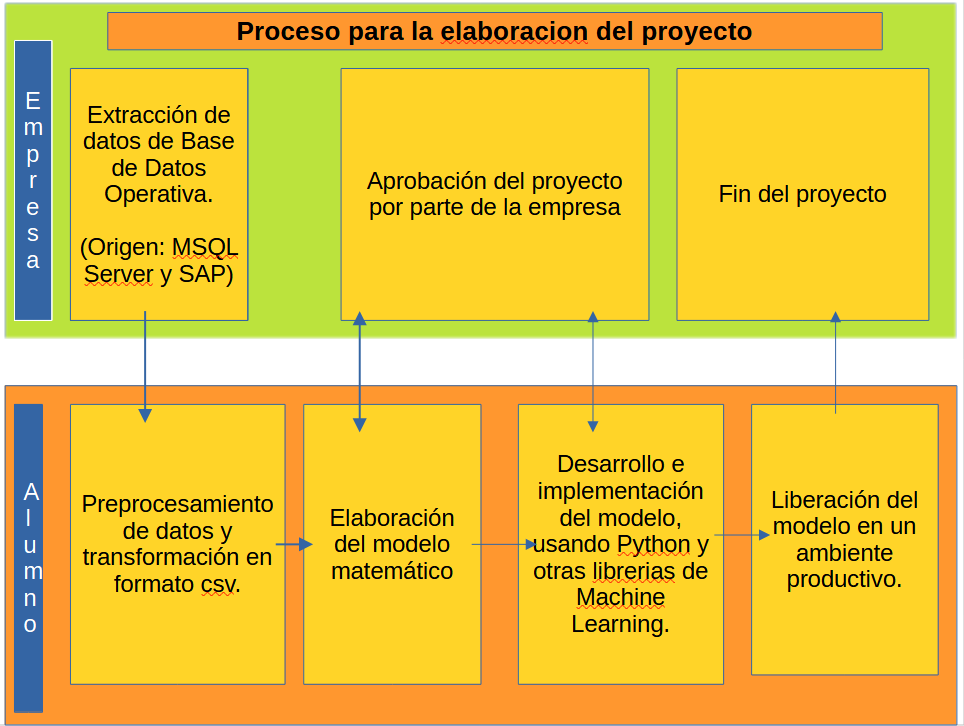
\includegraphics[width=12cm, height=7cm ]{Imagenes/Proceso_Proyecto.PNG }
      \caption{Metodología}
      \label{fig:meto}
\end{figure}

La metodología para realizar el proyecto se explica con la figura anterior.

\begin{itemize}
    \item La empresa proporciona la información con la que quiere que se desarrolle el modelo en formato Excel. \medskip
    \item Se recibe el archivo Excel y se realiza la limpieza y preprocesamiento de datos y se convierte a un formato de texto CSV , para usarlo como entrada por el algoritmo de aprendizaje . \medskip
    \item Se elabora el modelo y se interactúa con la empresa , hasta lograr un modelo este de acuerdo a sus necesidades. \medskip
    \item Una vez aprobado el modelo, se desarrolla el algoritmo usando el lenguaje de programación Python y otras librerías adicionales.\medskip
    \item El script o programa es evaluado por la empresa, la cual da su aprobación en cuanto a la funcionalidad requerida. \medskip
    \item Completado el anterior paso la empresa da su aprobación, con lo cual queda concluido el proyecto terminal. \medskip 
\end{itemize}

Una parte de dataset de trabajo es el siguiente :

\begin{figure}[H]
    \centering
       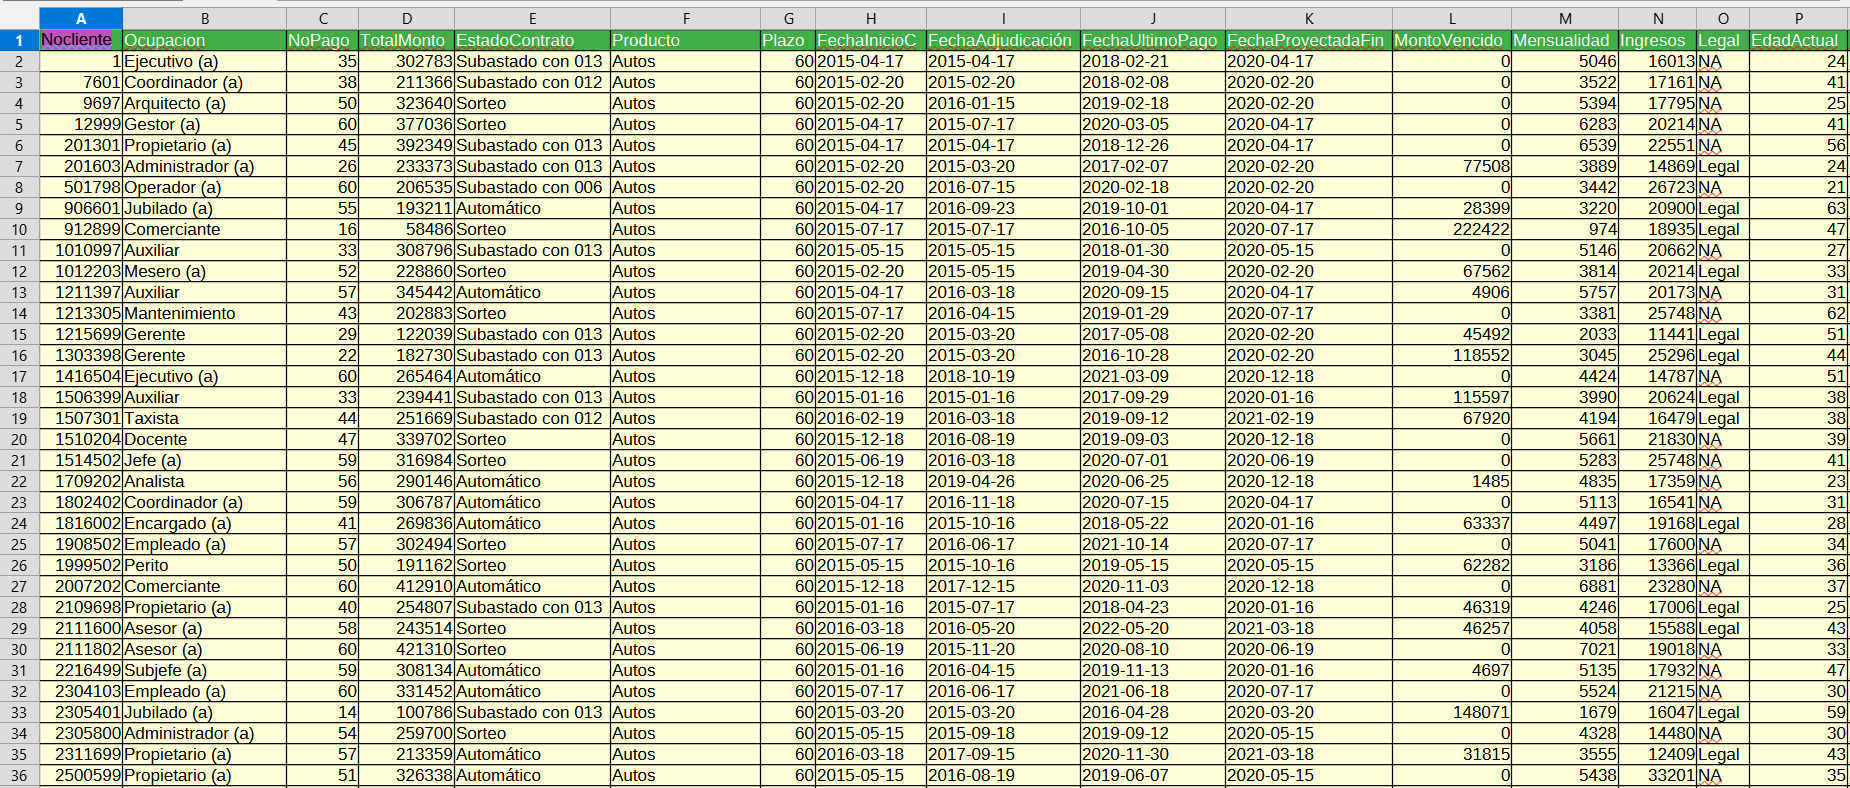
\includegraphics[width=12cm, height=10cm ]{Imagenes/Datos_Clientes1.PNG }
      \caption{Datos de los clientes (Bloque 1)}
      \label{fig:clis1}
\end{figure}
\newpage
\begin{figure}[H]
    \centering
       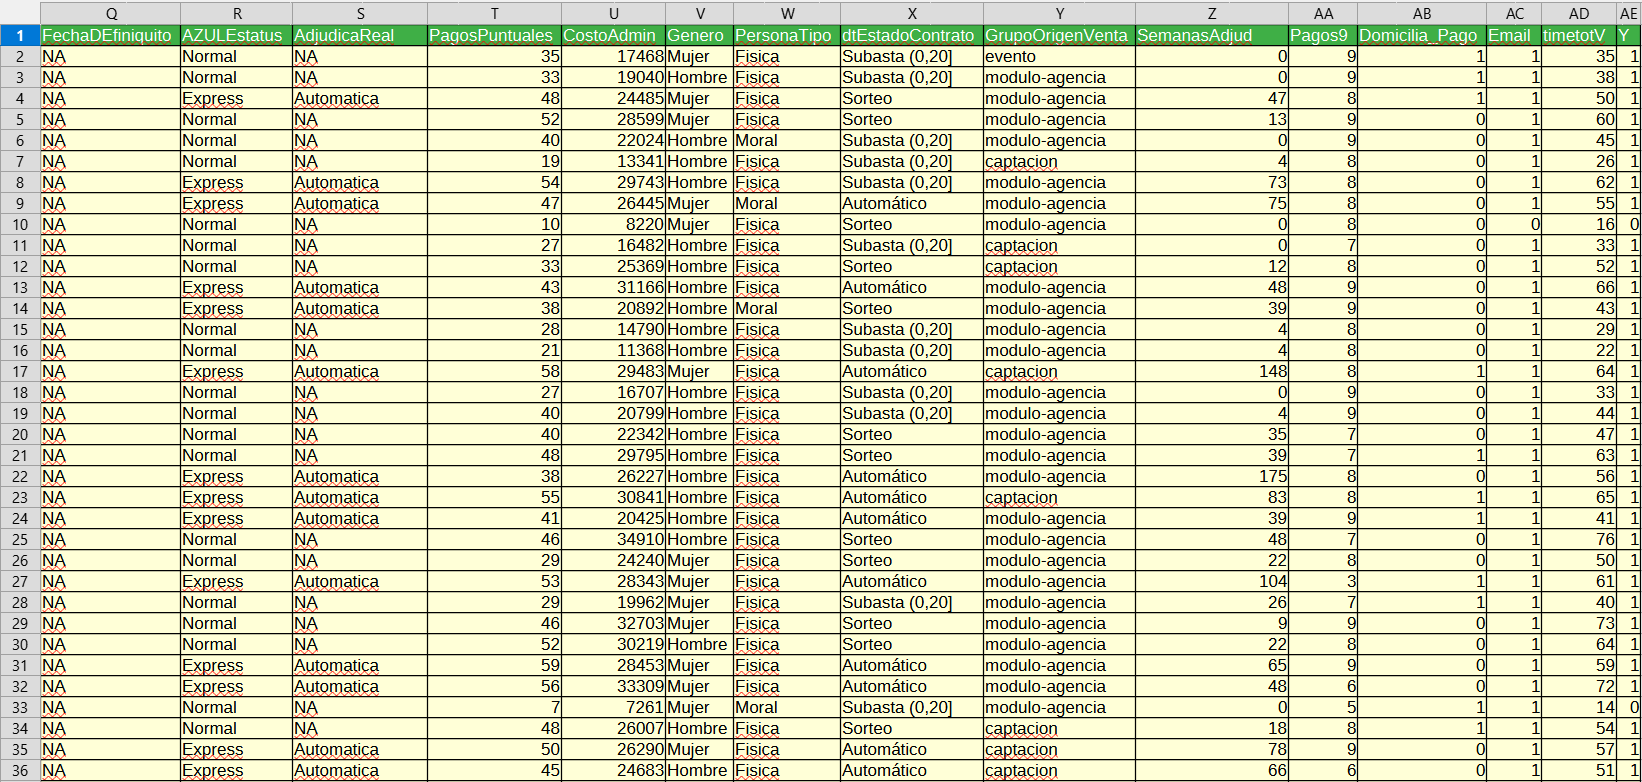
\includegraphics[width=12cm, height=10cm ]{Imagenes/Datos_Clientes2.PNG }
      \caption{Datos de los clientes (Bloque 2)}
      \label{fig:clis2}
\end{figure}
 
Descripción de las variables :

\begin{table}[H]
    \centering
    \begin{tabular}{|c|c|c|}
        \hline
        \rowcolor{softblue} % Fila color azul suave
        \textbf{Num} & \textbf{Nombre} & \textbf{Descripción} \\
        \hline
        % \rowcolor{lightgray} % Fila color gris claro
        \hline
        0 &	Nocliente &		Numero de cliente unico.   \\
        \hline
        1 &	Ocupacion &		Ocupación o profesión del cliente. 	\\
        \hline
        2 &  NoPago    &     Numero de pago actual. Entre 1 y 60 meses.  \\
        \hline
        3 &  TotalMonto  &    Cantidad  en moneda nacional, que se le prestó al cliente. \\
        \hline
        4 &  EstadoContrato &     Automático, Sorteo o Subasta.  \\
        \hline
        5 &   Producto  &         Auto, Inmueble, Moto (inicalmente solo se trabaja con Auto).  \\
        \hline
        6 &  Plazo     &          60 meses.  \\
        \hline
        7 &  FechaInicioC  &      Fecha de inicio de contrato.  \\
        \hline
        8 &  FechaAdjudicación &   Fecha de adjudicación del Auto.  \\
        \hline
        9 &   FechaUltimoPago &    Fecha de ultimo pago del prestamo. \\
        \hline
        10 &  FechaProyectadaFin &  Fecha proyectada de ultimo pago. \\
        \hline
        11 &  MontoVencido &        Monto vencido de pago.  \\
        \hline
        12 &  Mensualidad &         Cantidad a pagar mensualmente.  \\
        \hline
        % \rowcolor{mediumgray}
        13 &  Ingresos &    Ingreso mensual del cliente.  \\
        \hline
        % \rowcolor{mediumgray}
        14 &  Legal &     Si esta en estado normal o legal. \\
        \hline
        15 &  EdadActual &   Edad actual del cliente. \\
        \hline
        %\rowcolor{mediumgray}
        16 &  FechaDEfiniquito &    Fecha de finiquito. \\
        \hline
        17 &  AZULEstatus &   Express , normal. \\
        \hline
        %\rowcolor{mediumgray}
        18 &  AdjudicaReal &  Automática, normal , automática plus.\\
        \hline
        19 &  PagosPuntuales &      Numero de pagos puntuales en meses.  \\
        \hline
        20 &  CostoAdmin &    Costo administrativo por cliente. \\
        \hline
        21 &  Genero &       Mujer, Hombre u Otro . \\
        \hline
        22 &  PersonaTipo &   Si es persona física o moral. \\
        \hline
        23 &  dtEstadoContrato &    Automático , subasta, sorteo. \\
        \hline
        24 &  GrupoOrigenVenta &    Modulo-agencia, captación , facebook, telmkt, web , evento .\\
        \hline
        25 &  SemanasAdjud &    Semanas antes de adjudicación.  \\
        \hline
        26 &  Pagos9 &    Numero de pagos realizados antes del noveno pago. \\
        \hline
        27 &  DomiciliaPago &   Si el cargo se le realiza en tarjeta de credito. \\
        \hline
        28 &  Email &      Si cuenta con e-mail (1=si , 0=no). \\
        \hline
        29 &  timetotV &  Meses estimados de pago. Depende de pagos no puntuales. \\
        \hline
        30 &  Y &  Etiqueta binaria. Clasifica al cliente (0= No cofiable,1=confiable). \\
        \hline  
    \end{tabular}
    \caption{Descripción de las variables numéricas y categóricas}
\end{table} \medskip
\section{Limpieza del dataset y análisis exploratorio preliminar}

La limpieza de datos es una etapa esencial en el proceso de machine learning porque garantiza 
que el modelo trabaje con información de calidad, lo que mejora la precisión de sus resultados. 
Con frecuencia, los datos originales contienen errores, valores faltantes, duplicados o ruido, 
lo cual puede desviar el análisis y llevar a conclusiones equivocadas. Al procesar y limpiar los 
datos, se eliminan estas imperfecciones, ayudando a que el modelo se enfoque en patrones verdaderos
en lugar de anomalías. \medskip

La limpieza también permite identificar y gestionar los valores atípicos o outliers, que pueden 
distorsionar los resultados si no se manejan adecuadamente. Además, durante el proceso de 
limpieza, los datos se estandarizan y normalizan, especialmente cuando las variables presentan 
diferentes escalas o unidades; esto evita sesgos en el entrenamiento del modelo. \medskip

El programa o script para la limpieza de datos lo podemos ver almacenado en GitHub en el siguiente link \cite{roh1} . \medskip

Despues de cargar el dataset,mostraremos y verificaremos que es la información con la que vamos a trabajar : \medskip

\begin{figure}[H]
    \centering
       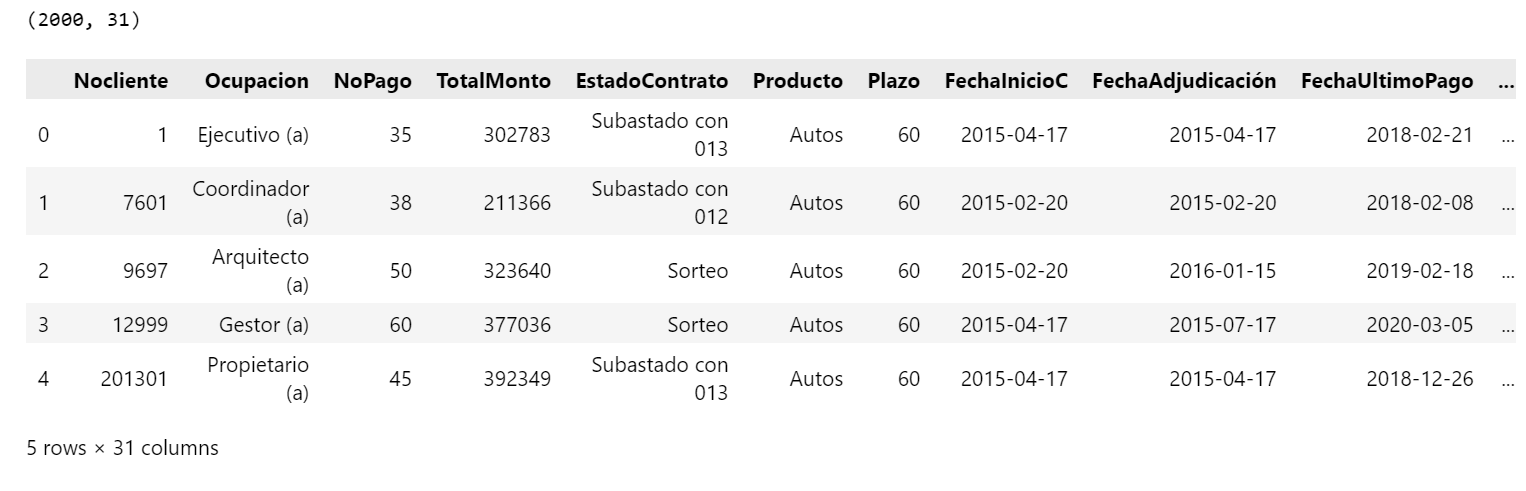
\includegraphics[width=14cm, height=8cm ]{Imagenes/DatasetLeido.PNG }
      \caption{Conjunto de datos o dataset leido}
      \label{fig:datasetl}
\end{figure}



Comenzaremos viendo las variables categóricas y numéricas usando la libreria Pandas y Python. Obtenemos la siguiente información como respuesta
\newpage
\begin{verbatim}
RangeIndex: 2000 entries, 0 to 1999 
Data columns (total 31 columns):
\end{verbatim}

\begin{table}[H]
    \centering
    
    \begin{tabular}{|c|c|c|c|c|}
        \hline
        \rowcolor{softblue} % Fila color azul suave
        \textbf{Num} & \textbf{Columna} & \textbf{Count} & \textbf{Non-Null} & \textbf{Dtype} \\
        \hline
        % \rowcolor{lightgray} % Fila color gris claro
        \hline
        0 &	Nocliente &		2000 &	non-null &	int64  \\
        \hline
        1 &	Ocupacion &		2000 &	non-null &	object \\
        \hline
        2 &  NoPago    &          2000 & non-null &  int64  \\
        \hline
        3 &  TotalMonto  &        2000 & non-null &  int64  \\
        \hline
        4 &  EstadoContrato &     2000 & non-null &  object \\
        \hline
        5 &   Producto  &         2000 & non-null &   object \\
        \hline
        6 &  Plazo     &          2000 & non-null &   int64  \\
        \hline
        7 &  FechaInicioC  &      2000 & non-null &   object \\
        \hline
        8 &  FechaAdjudicación &   2000 & non-null &   object \\
        \hline
        9 &   FechaUltimoPago &     2000 & non-null &   object \\
        \hline
        10 &  FechaProyectadaFin &  2000 & non-null &   object \\
        \hline
        11 &  MontoVencido &        2000 & non-null &   int64  \\
        \hline
        12 &  Mensualidad &         2000 & non-null &   int64  \\
        \hline
        \rowcolor{mediumgray}
        13 &  Ingresos &            1958 & non-null &   float64 \\
        \hline
        \rowcolor{mediumgray}
        14 &  Legal &               520 & non-null &    object \\
        \hline
        15 &  EdadActual &          2000 & non-null &   int64  \\
        \hline
        \rowcolor{mediumgray}
        16 &  FechaDEfiniquito &    0 & non-null &      float64 \\
        \hline
        17 &  AZULEstatus &         2000 & non-null &   object \\
        \hline
        \rowcolor{mediumgray}
        18 &  AdjudicaReal &        1457 & non-null &   object \\
        \hline
        19 &  PagosPuntuales &      2000 & non-null &   int64  \\
        \hline
        20 &  CostoAdmin &          2000 & non-null &   int64  \\
        \hline
        21 &  Genero &              2000 & non-null &   object \\
        \hline
        22 &  PersonaTipo &         2000 & non-null &   object \\
        \hline
        23 &  dtEstadoContrato &    2000 & non-null &   object \\
        \hline
        24 &  GrupoOrigenVenta &    2000 & non-null &   object \\
        \hline
        25 &  SemanasAdjud &        2000 & non-null &   float64 \\
        \hline
        26 &  Pagos9 &              2000 & non-null &   int64  \\
        \hline
        27 &  DomiciliaPago &      2000 & non-null &   int64  \\
        \hline
        28 &  Email &               2000 & non-null &   int64  \\
        \hline
        29 &  timetotV &            2000 & non-null &   int64  \\
        \hline
        30 &  Y &                   2000 & non-null &   int64 \\
        \hline  
    \end{tabular}
    \caption{Tabla con las variables numéricas y categóricas}
    \label{tab:vaxxx}
\end{table} \medskip

La tabla \ref{tab:vaxxx}  muestra que trabajaremos con un conjunto de datos de 2000 clientes y cada cliente con 30 columnas o variables. 
Además, nos indica la cantidad de información disponible en cada variable o columna. 
Si el tipo de dato (Dtype) es ''object'', la columna es categórica; de lo contrario, es una variable numérica.\medskip

Las variables numéricas son (int64 , float64):\medskip

NoPago, TotalMonto, MontoVencido, Mensualidad, Ingresos, EdadActual, CostoAdmin, SemanasAdjud,  Pagos9, Domicilia\_Pago, Email, timetotV \medskip

Y las variables categóricas (object):\medskip

Ocupacion, EstadoContrato, Producto, Legal, AZULEstatus,AdjudicaReal, Genero, PersonaTipo, dtEstadoContrato, GrupoOrigenVenta \medskip

Seguiremos los siguientes pasos sugeridos por Bronwnle J. \cite{Brown1} : \medskip
\begin{itemize}
    \item Eliminación de columnas con un único valor.
    \item Consideración de columnas con pocos valores únicos.
    \item Eliminación de columnas con baja variación.
    \item Identificación y eliminación de filas con datos duplicados.
    \item Eliminación de valores extremos (outliers) en caso de variables numéricas.
    \item Estandarización de errores tipográficos en variables categóricas.
\end{itemize}



\subsection{Eliminar columnas que contienen un solo valor} 

    La columna 'FechaDEfiniquito' no contiene información , ademas la columna 'Plazo' 
    solo tiene un valor y 'Nocliente' no es necesario, por lo que las eliminamos.
    

\subsection{ Considerar y/o eliminar columnas que tienen muy pocos valores}

En la tabla \ref{tab:vaxxx} vemos las variables que tienen menos información en un color gris mas oscuro. \medskip

Completamos y corregimos estas columnas usando las siguientes reglas del negocio: \medskip

\begin{itemize}
    \item Si el ingreso del cliente es menor o igual a 3,500 pesos, subimos a $ 4 * 3,500 $.
    \item La edad de cliente debe ser siempre mayor o igual a 18 años.
    \item La mensualidad debe ser siempre menor o igual ingreso.
    \item La variable o columna Legal debe tener uno de los valores Legal o Normal.
\end{itemize}

\subsection{ Identificar y eliminar filas duplicadas}

Dado que los clientes tienen un numero unico asignado, este proceso no se realiza. \medskip
\subsection{ Eliminación de valores extremos (outliers) en caso de variables numéricas}

En la siguiente tabla podemos ver los valores fuera de rango o outliers. \medskip
\newpage
\begin{figure}[H]
    \centering
       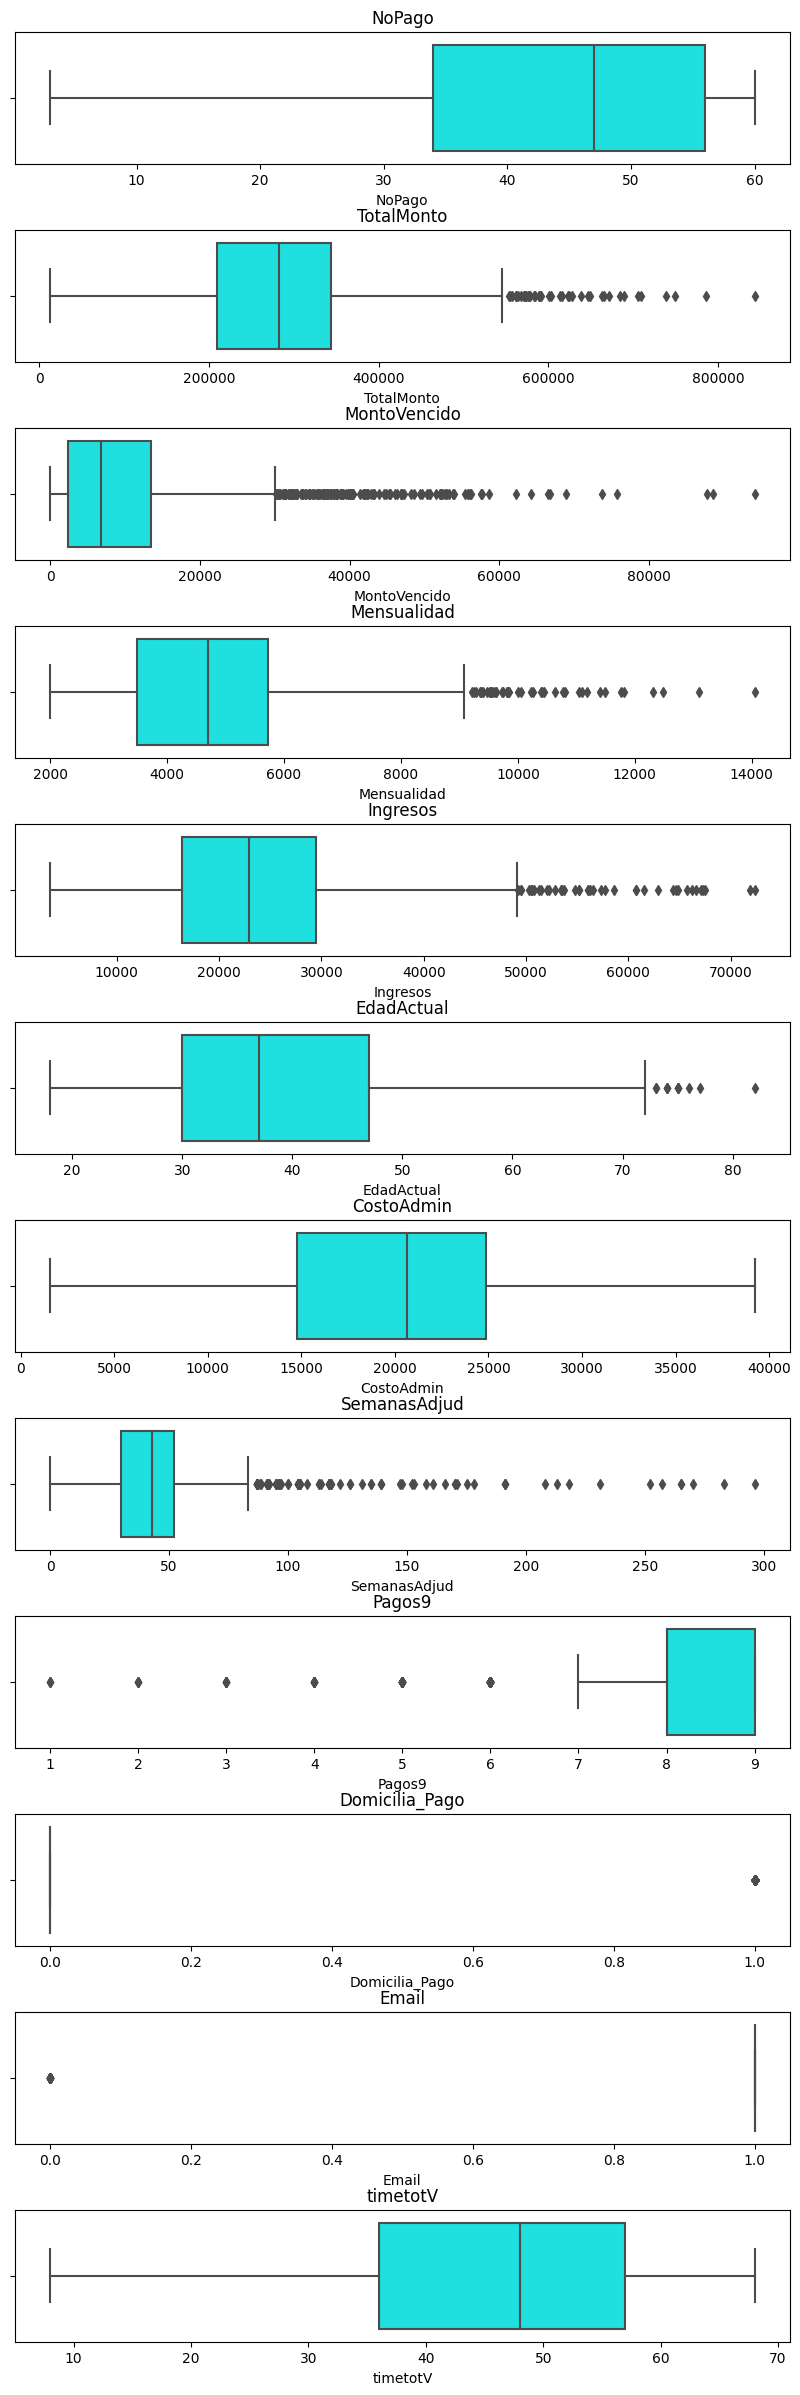
\includegraphics[width=16cm, height=21cm ]{Imagenes/GraficaCajaYBigoteNumericas.png}
      \caption{Valores fuera de rango o outliers}
      \label{fig:Outliers}
\end{figure}

De la figura \ref{fig:Outliers} consideramos que los valores numéricos fuera de rango son aceptables.

Las variables categóricas se ponen en minúsculas y en la figura \ref{fig:NivelesCate} , podemos observar 
los niveles o valores distintos que toma una variables categórica. \medskip
\begin{figure}[H]
    \centering
       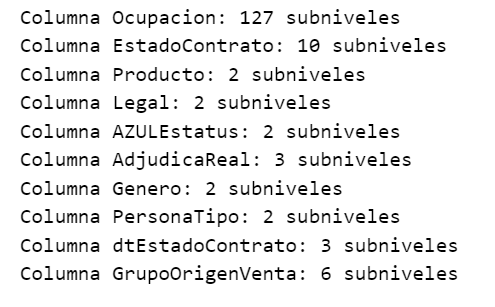
\includegraphics[width=12cm, height=5cm ]{Imagenes/SubNivelesCategoricas.PNG}
      \caption{Niveles o valores que toma una variables categórica}
      \label{fig:NivelesCate}
\end{figure}

Se detecta cualquier anomalía mediante las graficas de barras de cada una de ellas.\medskip

\begin{figure}[H]
    \centering
       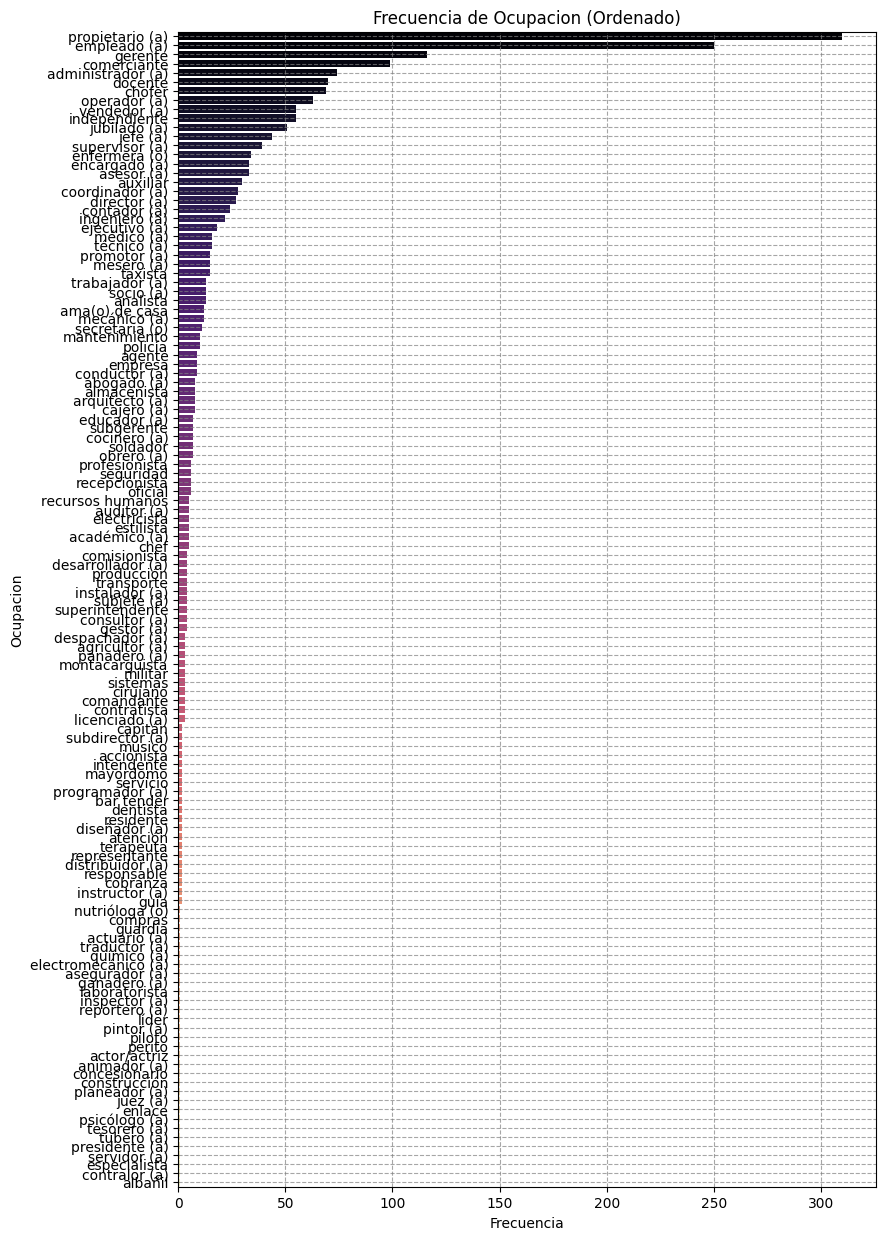
\includegraphics[width=14cm, height=21cm ]{Imagenes/Ocupacion.png}
      \caption{Grafica de ocupación del cliente vs frecuencia}
      \label{fig:Ocupacion}
\end{figure}

\begin{figure}[H]
    \centering
       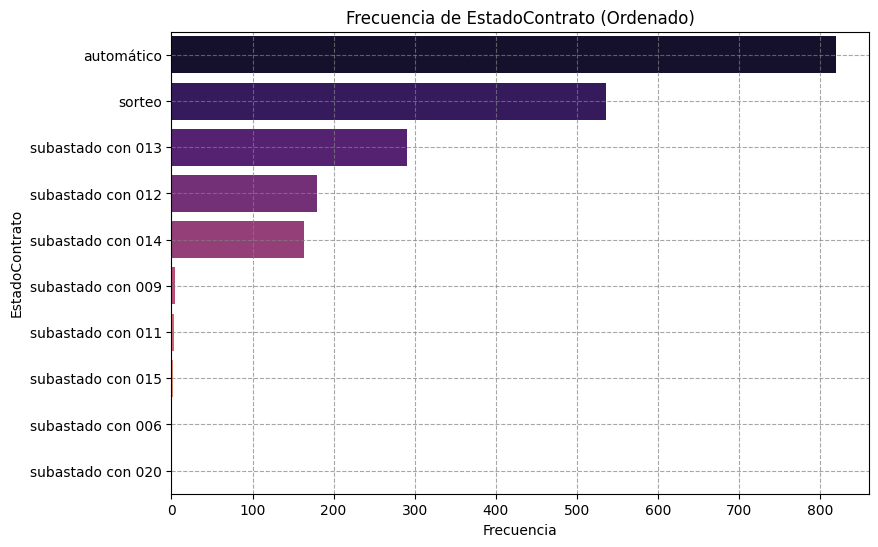
\includegraphics[width=14cm, height=10cm ]{Imagenes/EstadoContrato.png}
      \caption{Grafica de estado de contrato  vs frecuencia}
      \label{fig:Edocontra}
\end{figure}
\begin{figure}[H]
    \centering
       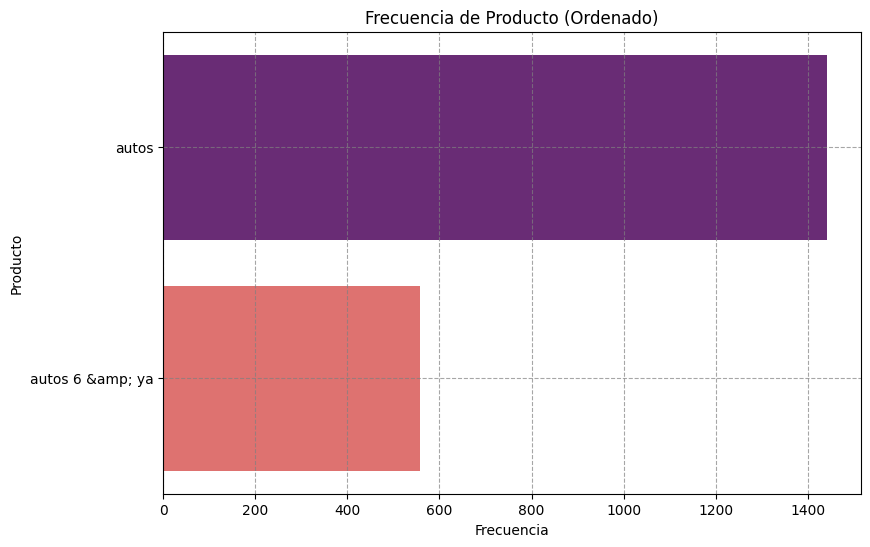
\includegraphics[width=14cm, height=10cm ]{Imagenes/Producto.png}
      \caption{Grafica de producto  vs frecuencia}
      \label{fig:ProductoF}
\end{figure}

\section{Medidas Estadísticas}

Determinamos la estadística básica del dataset, calculando para las variables numéricas

\begin{itemize}
    \item Promedio (mean).
    \item Desviación estandard (std).
    \item Valor mínimo.
    \item Valor máximo.
    \item Cuartiles (25\%, 50\% y 75\%).
\end{itemize} \medskip


\begin{figure}[H]
    \centering
       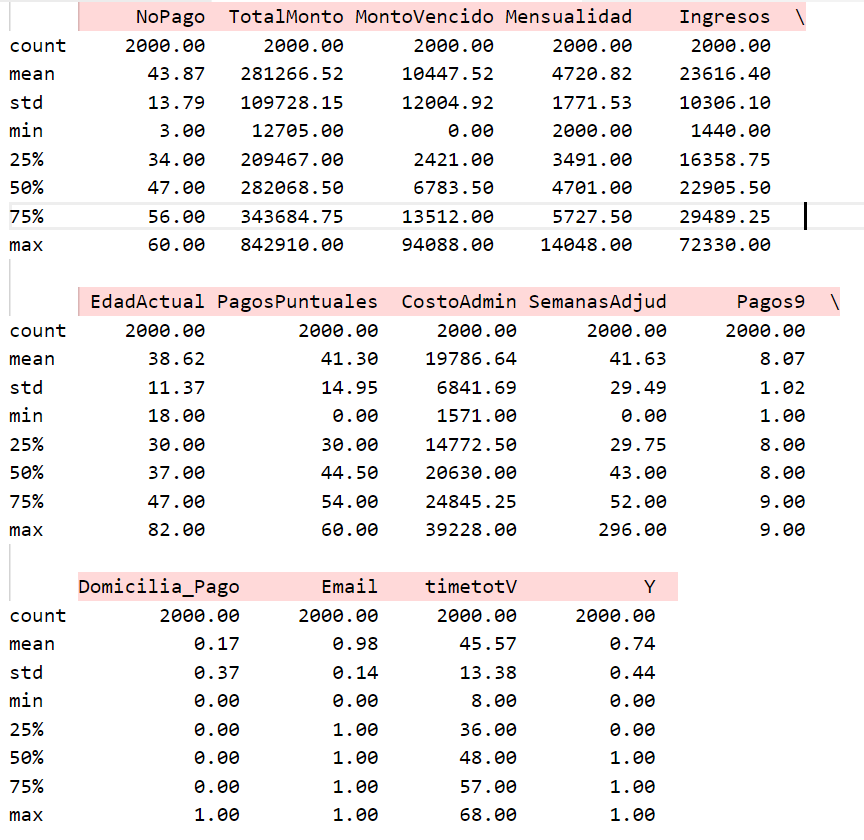
\includegraphics[width=14cm, height=16cm ]{Imagenes/EstadisticaBasica.PNG}
      \caption{Estadística básica para variables numéricas}
      \label{fig:EstBasica}
\end{figure}

\section{Correlación entre variables}

\begin{figure}[H]
    \centering
       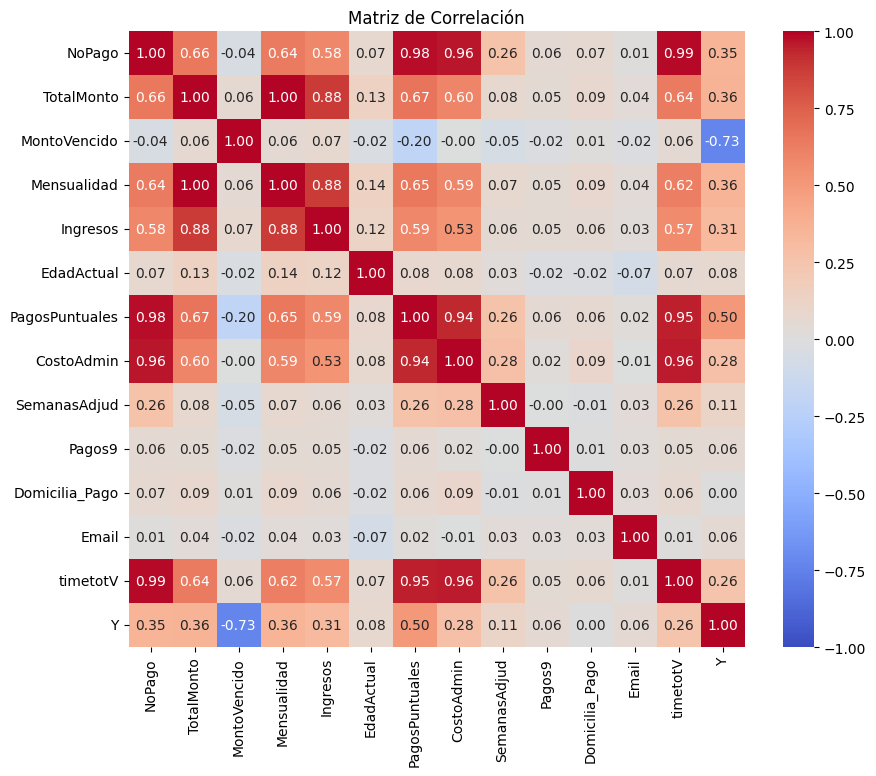
\includegraphics[width=14cm, height=14cm ]{Imagenes/Correlaciones.png}
      \caption{Correlaciones entre variables numéricas}
      \label{fig:Corres}
\end{figure}

Finalmente se guarda el dataset limpio en el archivo : ``Clientes\_Dos\_Mil\_Limpio.csv''.


\section{Transformación del dataset}
Para que un algoritmo de machine learning funcione bien, es crucial que los datos de entrada estén 
en el formato adecuado. En la mayoría de los casos, estos algoritmos requieren datos en formato 
numérico para realizar sus cálculos.\medskip

El proceso de adaptar o transformar los datos para que sean compatibles con el algoritmo se llama 
preprocesamiento y transformación de datos.

\subsection{Transformación StandardScaler}
Es el proceso mediante el cual un conjunto de datos se transforma para que siga una distribución normal
con media 0 y desviación estándar 1. \medskip

Matemáticamente : $ x_i' = \displaystyle {\frac{x_i - \mu}{\sigma}} $ \medskip

Con scikit-learn : \medskip

\begin{tcolorbox}[colback=gray!30, coltext=black, colframe=black, boxrule=0.5mm, width=\textwidth]
    \begin{verbatim}
        from sklearn.preprocessing import StandardScaler
        X_transformado = StandardScaler().fit_transform(X)
    \end{verbatim}
\end{tcolorbox}

De forma grafica podemos ver en la siguiente figura \ref{fig:crudoAstandar} , en que consiste la transformación

\begin{figure}[h!]
    \centering
    \begin{minipage}{0.45\textwidth}
        \centering
        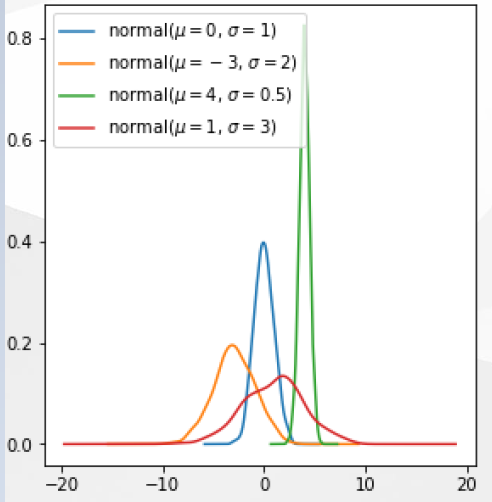
\includegraphics[width=\linewidth]{Imagenes/StandarCrudo.PNG}
        \caption{Datos en crudo}
        \label{fig:DatosCru}
    \end{minipage}
    \hspace{0.05\textwidth}
    \begin{minipage}{0.45\textwidth}
        \centering
        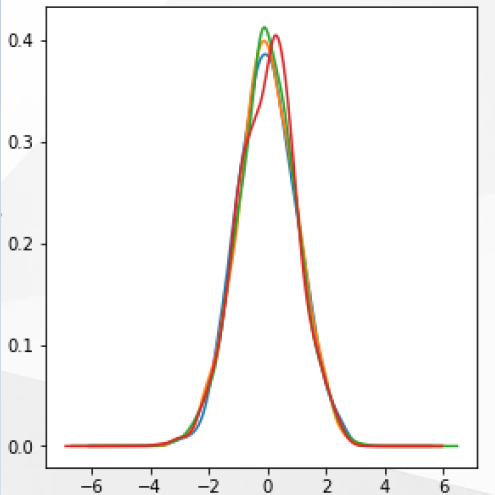
\includegraphics[width=\linewidth]{Imagenes/StandarNormalizado.PNG}
        \caption{StandardScaler}
        \label{fig:figura2}
    \end{minipage}
    \caption{Transformación de datos en crudo a StandardScaler}
    \label{fig:crudoAstandar}
\end{figure}

\subsection{Transformación OrdinalEnconder}

OrdinalEncoder asigna un valor numérico ordinal a cada categoría. De forma predeterminada, 
estos valores se asignan siguiendo el orden alfabético de las categorías. \medskip

Con scikit-learn : \medskip

\begin{tcolorbox}[colback=gray!30, coltext=black, colframe=black, boxrule=0.5mm, width=\textwidth]
    \begin{verbatim}
        from sklearn.preprocessing import OrdinalEncoder
        datos_transformados = encoder.fit_transform(datos)
    \end{verbatim}
\end{tcolorbox}

De forma grafica podemos ver en la siguiente figura \ref{fig:Orencoder} , la transformación de una
variable categórica a OrdinalEnconder. \medskip

\begin{figure}[H]
    \centering
       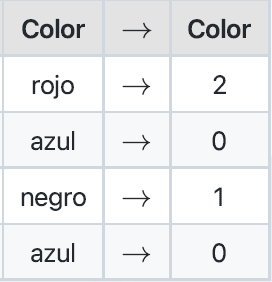
\includegraphics[width=4cm, height=5cm ]{Imagenes/Encoder.PNG}
      \caption{Transformación de una variable categórica a OrdinalEncoder}
      \label{fig:Orencoder}
\end{figure}

\section{Partición del dataset}

    \begin{figure} [H]
        \centering
        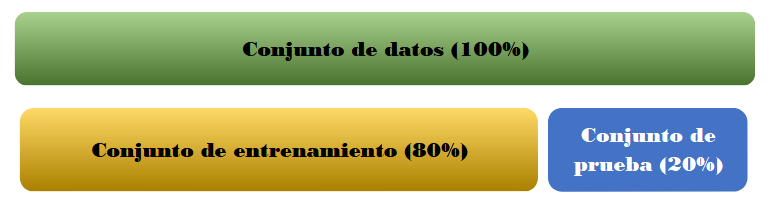
\includegraphics[width=12cm, height=4cm ]{Imagenes/ParticionDEdatos.PNG }
        \caption{Partición del dataset}
        \label{fig:parti}
    \end{figure}

    

\subsection{Partición del dataset}



